\documentclass[aspectratio=169]{beamer}

\usepackage{amsmath}
\usepackage{booktabs}
\usepackage[english]{babel}
\usepackage{unicode-math}
\usepackage{mathtools}
\usepackage{derivative}
\usepackage{makecell}
\usepackage{siunitx}

\usetheme{metropolis}

\setmainfont{Stix Two Text}
\setmathfont{Stix Two Math}

\DeclarePairedDelimiter{\ceil}{\lceil}{\rceil}
\DeclarePairedDelimiter{\floor}{\lfloor}{\rfloor}
\DeclarePairedDelimiter{\abs}{\lvert}{\rvert}
\DeclarePairedDelimiter{\norm}{\lVert}{\rVert}
\DeclarePairedDelimiter{\bra}{\langle}{\rvert}
\DeclarePairedDelimiter{\ket}{\lvert}{\rangle}
\DeclarePairedDelimiter{\expval}{\langle}{\rangle}
\DeclarePairedDelimiter{\norder}{\mathcolon}{\mathcolon}
\DeclarePairedDelimiter{\anorder}{\typecolon}{\typecolon}
	
\newcommand{\laplace}{\mbfnabla^2}
\newcommand{\trans}{{\scriptscriptstyle\mathsf{T}}}

\newcommand{\conv}{\ast}
\newcommand{\vdot}{\cdot}
\newcommand{\vcross}{\vectimes}
\newcommand{\vb}[1]{\symbfup{#1}}
\newcommand{\vu}[1]{\hat{\vb{#1}}}
\newcommand*\dd[2][\relax]{\mathop{\ifx\relax#1\odif{#2}\else \odif[order={#1}]{#2}\fi}}

\newcommand{\vacket}{\ket*{0}}
\newcommand{\vacbra}{\bra*{0}}

\DeclareMathOperator{\trace}{Tr}
\DeclareMathOperator{\sinc}{sinc}

\AtBeginDocument{
	\let\Re\relax
	\let\Im\relax
	\DeclareMathOperator{\Re}{Re}
	\DeclareMathOperator{\Im}{Im}

	\renewcommand{\div}{\mathop{\mbfnabla\vdot}}
	\newcommand{\curl}{\mathop{\mbfnabla\vectimes}}
}

\DeclarePairedDelimiterX{\comm}[2]{[}{]}{#1,#2}

\DeclarePairedDelimiterX{\braket}[2]{\langle}{\rangle}{#1\delimsize\vert#2}
\DeclarePairedDelimiterX{\ketbra}[1]{\lvert}{\rvert}{#1\rangle\delimsize\langle#1}


\usetikzlibrary{arrows.meta,fit,mindmap,positioning}

\title{A theoretical framework for CV-QKD}
\date{\today}
\author{Bodo Kaiser}
\institute{Ludwig-Maximilians-Universität München}

\begin{document}
	\maketitle
	
	\begin{frame}
		\begin{center}
			\textbf{Prelude}
			
			What is light?
		\end{center}
	\end{frame}
	
	\section{Introduction}

	% what is secure communication: integrity and confidentiality	
	% key distribution problem
	% public-key distribution
	% information-theoretical secure for OTP but practically one uses AES
	\begin{frame}{Secure communication}
		\begin{figure}
			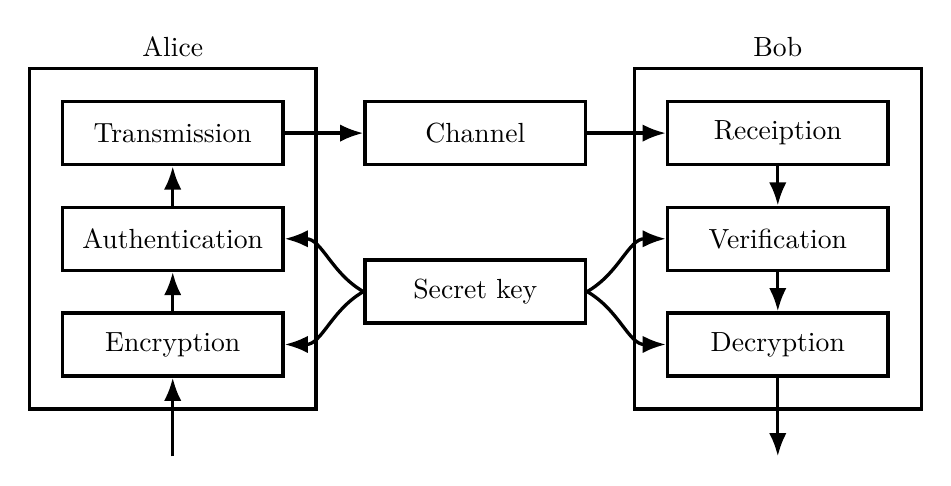
\begin{tikzpicture}[
				node distance=5mm,
				arrow/.style={very thick, -Latex},
				block/.style={draw, very thick, minimum width=28mm, minimum height=8mm},		
				superblock/.style={draw, very thick, inner sep=4mm},
			]
				\coordinate (in);
				\node[block, above=10mm of in] (encryption) {Encryption};
				\node[block, above=of encryption] (authentication) {Authentication};
				\node[block, above=of authentication] (transmitter) {Transmission};
				\node[block, right=10mm of transmitter] (channel) {Channel};
				\node[block, right=10mm of channel] (receiver) {Receiption};
				\node[block, below=of receiver] (verification) {Verification};
				\node[block, below=of verification] (decryption) {Decryption};
				\coordinate[below=10mm of decryption] (out);
	
				\path (encryption) -- (verification) node[midway, block] (key) {Secret key};
	
				\draw[arrow] (key.west) to[out=210, in=0] (encryption.east);
				\draw[arrow] (key.west) to[out=150, in=0]  (authentication.east);
				\draw[arrow] (key.east) to[out=-30, in=180] (decryption.west);
				\draw[arrow] (key.east) to[out=30, in=180] (verification.west);

				\draw[arrow] (in) -- (encryption);
				\draw[arrow] (encryption) -- (authentication);
				\draw[arrow] (authentication) -- (transmitter);
				
				\draw[arrow] (decryption) -- (out);
				\draw[arrow] (verification) -- (decryption);
				\draw[arrow] (receiver) -- (verification);
		
				\draw[arrow] (transmitter) -- (channel.west);
				\draw[arrow] (channel.east) -- (receiver);
				
				\node[superblock, label={Alice}, fit=(encryption) (transmitter)] {};
				\node[superblock, label={Bob}, fit=(decryption) (receiver)] {};
			\end{tikzpicture}
			\caption{Block diagram of a secure transmission system.}
		\end{figure}
	\end{frame}

	% main idea of QKD:
    % quantum transmission
	% post-processing	
	\begin{frame}{Quantum key distribution}
		\begin{figure}
			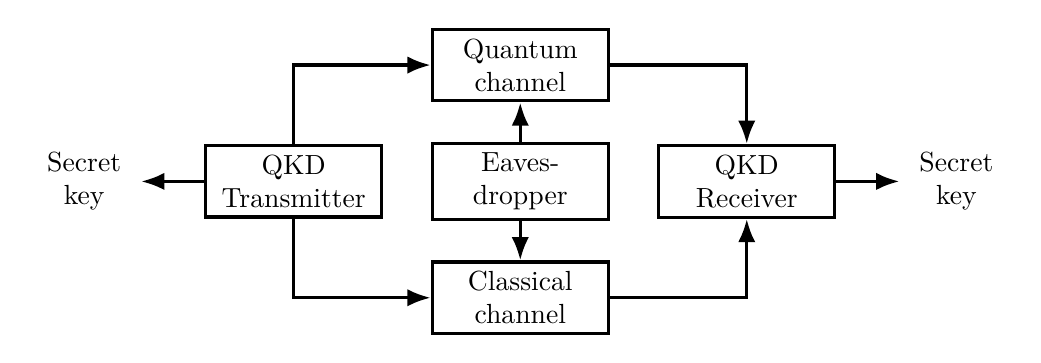
\begin{tikzpicture}[
				node distance=5mm,
				arrow/.style={very thick, -Latex},
				block/.style={draw, very thick, minimum width=20mm, minimum height=8mm, text width=20mm, align=center},
				superblock/.style={draw, very thick, inner sep=3mm},
			]
				\node[block] (transmitter) {QKD Transmitter};
				\node[text width=12mm, align=center, left=8mm of transmitter] (alice key) {Secret key};
	
				\node[block, right=6mm of transmitter] (eve) {Eavesdropper};
				\node[block, above=5mm of eve] (quantum channel) {Quantum channel};
				\node[block, below=5mm of eve] (classical channel) {Classical channel};
				\node[block, right=6mm of eve] (receiver) {QKD Receiver};
				\node[text width=12mm, align=center, right=8mm of receiver] (bob key) {Secret key};
				
				\draw[arrow] (transmitter) -- (alice key);
				\draw[arrow] (receiver) -- (bob key);
				\draw[arrow] (eve) -- (classical channel);
				\draw[arrow] (eve) -- (quantum channel);
				\draw[arrow] (transmitter.north) -- (transmitter.north|-quantum channel.west) -- (quantum channel.west);
				\draw[arrow] (transmitter.south) -- (transmitter.south|-classical channel.west) -- (classical channel.west);
				\draw[arrow] (quantum channel.east) -- (quantum channel.east-|receiver.north) -- (receiver.north);
				\draw[arrow] (classical channel.east) -- (classical channel.east-|receiver.south) -- (receiver.south);
				
				%\node[superblock, label={Alice}, fit=(alice key) (transmitter)] {};
				%\node[superblock, label={Bob}, fit=(bob key) (receiver)] {};
			\end{tikzpicture}
			\caption{Block diagram of a QKD system.}
		\end{figure}
	\end{frame}
	
	% why is QKD interesting? -> intersection of multiple disciplines (quantum information theory, quantum optics, communication engineering)
	\begin{frame}
		\begin{figure}
			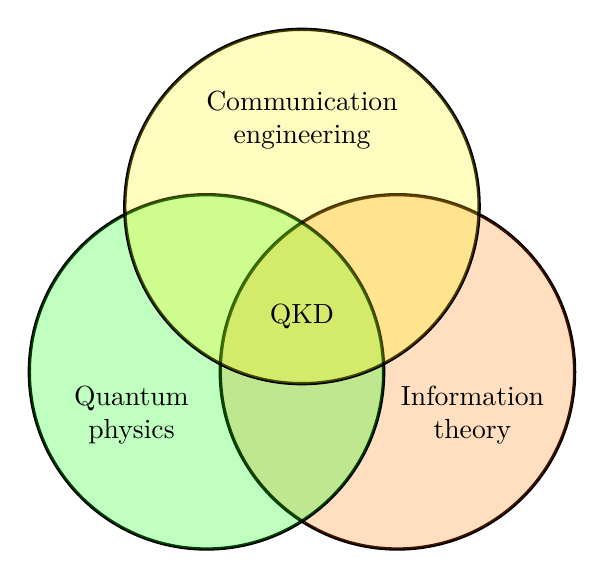
\begin{tikzpicture}[
				venn circle/.style={draw, very thick, fill opacity=0.25, circle, minimum width=45mm},
				venn label/.style={align=center},
			]
				\begin{scope}[blend group=soft light]
					\node[venn circle, fill=yellow] (qp) at (90:1.4) {};
					\node[venn circle, fill=green] (it) at (210:1.4) {};
					\node[venn circle, fill=orange] (qp) at (330:1.4) {};
				\end{scope}
				
				\node[venn label] {QKD};
				\node[venn label] at (90:2.5) {Communication\\engineering};
				\node[venn label] at (210:2.5) {Quantum\\physics};
				\node[venn label] at (330:2.5) {Information\\theory};
			\end{tikzpicture}
			\caption{Venn diagram of the disciplines contributing to QKD.}
		\end{figure}
	\end{frame}
	
	\begin{frame}{Taxonomy of QKD protocols}
		\begin{table}
			\caption{Summary of common characteristics among QKD protocols.}
			\begin{tabular}{lc}
				\toprule
				Protocol parameter & Typical options \\
				\midrule
				Schema & Entanglement-based or prepare-and-measure \\
				Detection & Coherent or single-photon \\
				\makecell[l]{Measurement-\\basis selection} & Active or passive \\
				Logical encoding & Qubit or Boson \\
				Physical encoding & Polarization, quadratures, squeezing, ... \\
				\bottomrule
			\end{tabular}
		\end{table}
	\end{frame}
	
	\begin{frame}{Qubit-based QKD}
		\begin{columns}[T, onlytextwidth]
			\column{0.4\textwidth}
			\begin{figure}
				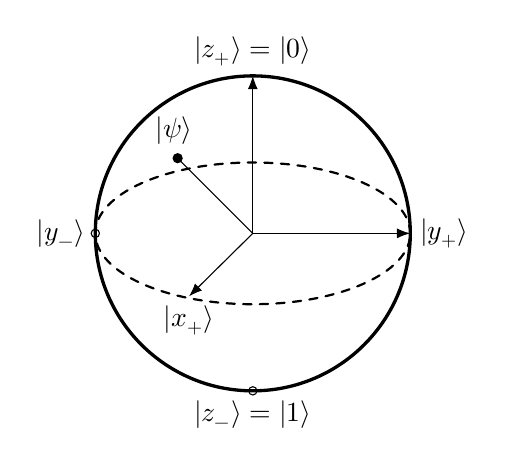
\begin{tikzpicture}[line cap=round, line join=round]
					\draw[very thick] (0,0) circle (2cm);
					\draw[thick, rotate around={0.:(0.,0.)}, dash pattern=on 3pt off 3pt] (0,0) ellipse (2cm and 0.9cm);
					\draw[-Circle] (0,0) -- (-1,1) node[above]{$\ket{\psi}$};
			
					\draw[-Latex] (0,0) -- (0,2) node[above]{$\ket{z_+}=\ket{0}$};
					\draw[-Latex] (0,0) -- (-0.81,-0.8) node[below]{$\ket{x_+}$};
					\draw[-Latex] (0,0) -- (2,0) node[right]{$\ket{y_+}$};
			
					\draw (0,-2) circle (1.5pt) node[below] {$\ket{z_-}=\ket{1}$};
					\draw (-2,0) circle (1.5pt) node[left] {$\ket{y_-}$};
				\end{tikzpicture}
				\caption{Bloch sphere with pure quantum state $\ket{\psi}=c_1\ket{0}+c_2\ket{1}$.}
			\end{figure}
			\column{0.5\textwidth}
			\begin{table}
				\caption{Physical encodings or logical qubit.}
				\begin{tabular}{lcc}
					\toprule
					Physical encoding & \multicolumn{2}{c}{Standard basis $\ket{0},\ket{1}$} \\
					\midrule
					Polarization & Horizontal & Vertical \\
					Photon number & Vacuum & Photon \\
					Time binning & Early & Late \\
					Phase binning & \SI{0}{\degree} & \SI{180}{\degree} \\
					\bottomrule
				\end{tabular}
			\end{table}
		\end{columns}
	\end{frame}
	
	\begin{frame}{Squeezing-encoding boson-based QKD}
		
	\end{frame}
	
	\begin{frame}{Coherent-encoding boson-based QKD}
		
	\end{frame}
	
	\begin{frame}{Problem statement}
		Venn-diagram of disciplines
		and 
		conflict
	\end{frame}
	
	\section{Classical communication theory}
	
	\section{Quantum theory of light}
	
	\section{Quantum theory of electro-optics}
	
	\section{Quantum communication theory}
	
	\section{Conclusion}
	
	\begin{frame}
		\begin{center}
			\textbf{Postlude}
			
			How does light interact with matter?
		\end{center}
	\end{frame}
\end{document}